\documentclass[a4paper, 12pt]{article}
\usepackage[a4paper,top=1.5cm, bottom=1.5cm, left=1cm, right=1cm]{geometry}

% Работа с русским языком
\usepackage[utf8]{inputenc}
\usepackage{mathtext}                % русские буквы в формулах
\usepackage[english, russian]{babel} % локализация и переносы

\usepackage{graphicx}   % Вставка изображений
\usepackage{float}      % "Плавающие" изображения3
\usepackage{wrapfig}    % Обтекание фигур (таблиц, картинок и прочего)
\usepackage{subfig}
\graphicspath{ {./images/} }

\usepackage{tabularx}
\usepackage{multirow}
\usepackage{booktabs}
\usepackage{amsmath}
\usepackage{amsfonts}
\usepackage{indentfirst}
\usepackage{longtable}
\graphicspath{{pictures/}}
\usepackage{natbib}
\usepackage{bm}

\newcommand{\figref}[1]{(См. рис. \ref{#1})}
\newcommand{\secref}[1]{(См. раздел. \ref{#1})}

\newcommand{\e}[1]{\text{$\cdot10^{#1}$}}
\newcommand{\m}{\; м}
\newcommand{\mm}{\; мм}
\newcommand{\um}{\; мкм}
\newcommand{\A}{\; А}
\newcommand{\uV}{\; мкВ}
\newcommand{\cels}{\; ^\circ С}

%%% Колонтитулы
\usepackage{titleps}
\newpagestyle{main}{
	\setheadrule{0.4pt}
	\sethead{Отчёт о выполнении лабораторной работы 8.1}{}{}
	\setfootrule{0.4pt}                       
	\setfoot{ФРКТ МФТИ, 2024}{}{\thepage} 
}
\pagestyle{main}  

\begin{document}
    \begin{titlepage}
	\begin{center}
            {\large МОСКОВСКИЙ ФИЗИКО-ТЕХНИЧЕСКИЙ ИНСТИТУТ (НАЦИОНАЛЬНЫЙ ИССЛЕДОВАТЕЛЬСКИЙ УНИВЕРСИТЕТ)}
	\end{center}
 
	\begin{center}
		{\large Физтех-школа радиотехники и компьютерных технологий}
	\end{center}
	
	\vspace{8cm}
	{\LARGE
		\begin{center}
                {\bf Отчёт о выполнении лабораторной работы 8.1}\\
                Определение постоянных Стефана-Больцмана и Планка из анализа теплового излучения накаленного тела
		\end{center}
	}
	\vspace{4cm}
	\begin{flushright}
		{\Large Авторы: \\ 
        Тихонов Дмитрий Романович, \\ студент группы Б01-206а \\
        Павловский Кирилл Михайлович, \\ студент группы Б01-206а}
	\end{flushright}
	\vspace{4cm}
	\begin{center}
		\Large Долгопрудный, 2024
	\end{center}
    \end{titlepage}


    \section{Введение}

    \noindent \textbf{Цель работы:} исследовать с помощью оптического термометра с исчезающей нитью зависимость температуры раскалённой вольфрамовой нити от мощности, рассеиваемой в нити, подтвердить линейную зависимость энергетической светимости от четвёртой степени температуры тела $T^4$, определить постоянные Стефана-Больцмана и Планка, качественно исследовать излучение различных накалённых тел. \\

    \noindent \textbf{В работе используются:} оптический пирометр, модель абсолютно чёрного тела (АЧТ), блок питания, цифровые мультиметры GDM-8145, трубка с кольцами из материалов с разной излучательной способностью, лампа накаливания, неоновая лампочка
    
    \section{Теоретические сведения}
    
    \textit{Абсолютно чёрным телом (АЧТ)} называется тело, которое поглощает всё падающее на него излучение, но при этом само излучает энергию. 
	
    \textit{Потоком излучения} $\Phi$ называется мощность излучения, переносимая излучением через выбранную поверхность.
    $$
    \Phi = \frac{dE}{dt}
    $$
    где $E$ -- энергия, переносимая излучением.
	
    \textit{Плотностью потока излучения} $j(T)$ называется мощность излучения, переносимая излучением через единичную поверхность:
    $$
    j(T) = \frac{\Phi}{S}
    $$
	
    Согласно \textit{закону Стефана-Больцмана} интегральная плотность потока излучения связана с температурой тела формулой:
    \begin{equation}
        j(T) = \sigma T^4
        \label{eq:stefan_boltzman_law}
    \end{equation}
    где $\sigma$ -- постоянная Стефана-Больцмана. Согласно квантовой механике постоянная Стефана-Больцмана связана с другими мировыми константами соотношением:
	\begin{equation}
		\sigma = \frac{2 \pi^5 k_Б^4}{15 c^2 h^3}.
		\label{eq:const_stefan_boltzmann}
	\end{equation}
	
    Согласно квантовой механике АЧТ излучает неравномерно на разных частотах. Для описания излучения на определённой частоте используется \textit{спектральная плотность потока излучения}:
    
    $$
    j_T(\omega) = \frac{d j(T)}{d \omega}
    $$
    
    Спектральная плотность потока излучения АЧТ вычисляется по \textit{формуле Планка}:
    
    $$
    j_T(\omega) = \frac{\hbar}{\left(2 \pi c \right)^2} \frac{\omega^3}{\exp \left(\frac{\hbar \omega}{k_Б T}\right) - 1}
    $$
    
    Из данной формулы можно получить зависимость спектральной плотности потока излучения от длины волны, если учесть, что $j_T(\omega) d\omega = j_T(\lambda) d\lambda$:
    
    $$
    j_T(\lambda) = \frac{\hbar c^2}{\lambda^5}  \frac{1}{\exp \left(\frac{h c}{\lambda k_Б T}\right) - 1}
    $$
    
    Типичный график зависимости спектральной плотности потока излучения $j_T(\lambda)$ АЧТ приведён на рисунке \ref{img:j_T(lambda)}:
    
    \begin{figure}[H]
        \centering
        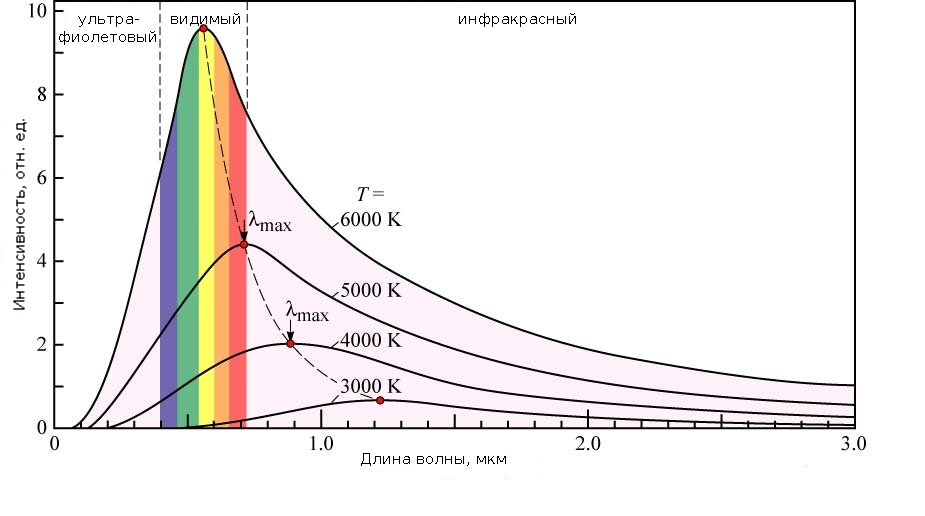
\includegraphics[width=1\textwidth]{images/j_t(lambda).jpg}
        \caption{График спектральной плотности потока излучения $j_T(\lambda)$ АЧТ для различных температур.}
        \label{img:j_T(lambda)}
    \end{figure}
    
    Спектральная плотность потока излучения имеет максимум $\lambda_{max}$. Формула, связывающая температуру тела и $\lambda_{max}$, называется \textit{законом смещения Вина}:
    $$
    T \lambda_{max} = 0,289776829 \dots \; К \cdot см
    $$

    \newpage
    
    \section{Методика измерений и экспериментальная установка}

    \subsection{Описание экспериментальной установки}

    Схема экспериментальной установки приведена на рисунке \ref{img:exp_scheme}:
    \begin{figure}[H]
        \centering
        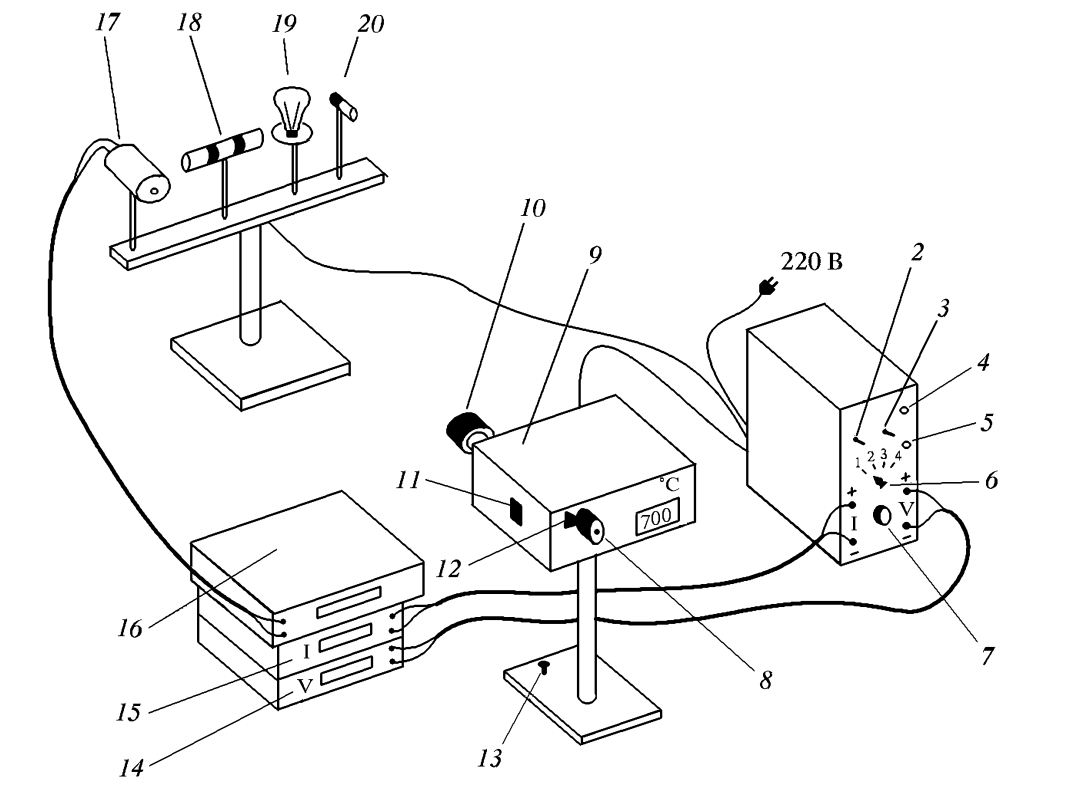
\includegraphics[width=1\textwidth]{images/exp_scheme.png}
        \caption{Схема экспериментальной установки}
        \label{img:exp_scheme}
    \end{figure}
	
    С помощью оптического пирометра с исчезающей нитью 9 измеряется яркостная температура исследуемого тела. Объектив 10 используется для получения чёткого изображения предмета. С помощью окуляра 8 настраивается чёткое изображение исчезающей нити. Задвижка 11 позволяет вводить в оптическую систему пирометра серый светофильтр для изменения измеряемого диапазона температур. Без светофильтра измеряются температуры в диапазоне $700 \div 1200 \cels$, со светофильтром -- в диапазоне $1200 \div 2000 \cels$. С помощью переключателя 12 в оптическую систему можно вводить красный светофильтр.
	
    В работе исследуется излучение четырёх тел (17-20), закреплённых на специальном стенде. Модель АЧТ 17 представляет собой керамическую трубку длиной $50 \mm$, диаметром $3 \mm$, закрытую с одного конца. Трубка окружена теплоизоляционным кожухом. Стенки трубки нагреваются намотанной на неё нихромовой спиралью. Дно трубки излучает практически как абсолютно чёрное тело. Температура дна измеряется с помощью хромель-алюмелевой термопары, один конец которой вмонтирован в дно трубки, а другой находится при комнатной температуре. ЭДС термопары измеряется вольтметром 16; 18 -- керамическая трубка с закрепленными на ней кольцами из разных материалов с разной излучательной способностью. Трубка нагревается изнутри проводом до температуры примерно $1100 \cels$ для качественного сравнения испускательной способности различных материалов. Лампочка накаливания с вольфрамовой нитью (19) используется для проверки закона Стефана-Больцмана и определения постоянных Планка и Стефана-Больцмана; 20 -- неоновая лампочка.
	
    Напряжение на исследуемые образцы подаётся с помощью блока питания, мощность регулируется ручкой 7, исследуемый образец можно выбирать с помощью переключателя 6. Напряжение на образце измеряется вольтметром 14, ток -- амперметром 15.

    \subsection{Оборудование и приборы}
		
    \begin{itemize}
        \item Оптический пирометр с исчезающей нитью Проминь М1. Диапазон измеряемых температур $800 \div 2000 \cels$, спектральный рабочий диапазон $\left( 0.655 \pm 0.001 \right) \um$. Оптимальное рабочее расстояние -- $0.7 \m$,
        
        \item Хромель-алюминиевая термопара. В диапазоне температур $900 \cels$ допустимое отклонение измеренной температуры от реальной составляет $\pm 7 \cels$, допустимое отклонение ЭДС $\pm 260 \uV$,
        
        \item Цифровые мультиметры GDM-8145. В режиме измерения постоянного напряжение погрешность измерения оценивается по формуле 
        
        $$
        \pm (0.03\% \cdot \text{<измеренное значение>} + 4 \text{ единицы младшего разряда}).
        $$
        
        В режиме измерения постоянной силы тока на пределе $20 \A$ допустимое отклонение измеренных значений от реальных составляет 
        $$
        \pm (0.3\% \cdot \text{<измеренное значение>} + 2\text{ единицы младшего разряда}),
        $$
        
        \item Лабораторный блок питания с возможность подключения различных образцов и регулируемой мощностью.
    \end{itemize}
	
    \subsection{Методика эксперимента}
	
    В начале работы проверяется, что пирометр правильно измеряет температуру. Для этого измеряется температура модели АЧТ с помощью термометра и термопары, показания приборов сверяются. ЭДС термопары $\varepsilon$ измеряется вольтметром и переводится в температуру $T_t$ согласно спецификации:
    $$
    T_t = \varepsilon / \psi + T_{л}
    $$
    где $\Psi = (41 \pm 1) \; мкВ/ ^\circ С$ -- постоянная термопары, $T_{л} = 25 \cels$ -- температура лаборатории.
	
    Для определение постоянной Стефана-Больцмана измеряется температура вольфрамовой нити и рассеиваемая в ней мощность. Предполагается, что в установившемся состоянии, вся подаваемая на вольфрамовую нить мощность $W$ рассеивается в виде излучения. Мощность $W$ определяется по закону Джоуля-Ленца и равна потоку излучения $\Phi$:
    
    $$
    \Phi = W = U \cdot I
    $$

    Пирометр измеряется \textit{яркостную температуру} нити. Под яркостной температурой понимается температура АЧТ, спектральная испускательная способность которого равна спектральной испускательной способности исследуемого тела на определённой длине волны. Для ограничения спектра излучения используется красный светофильтр пирометра. Для определения реальной температуры вольфрамовой нити по известной яркостной используется зависимость:
	
    \begin{figure}[H]
        \centering
        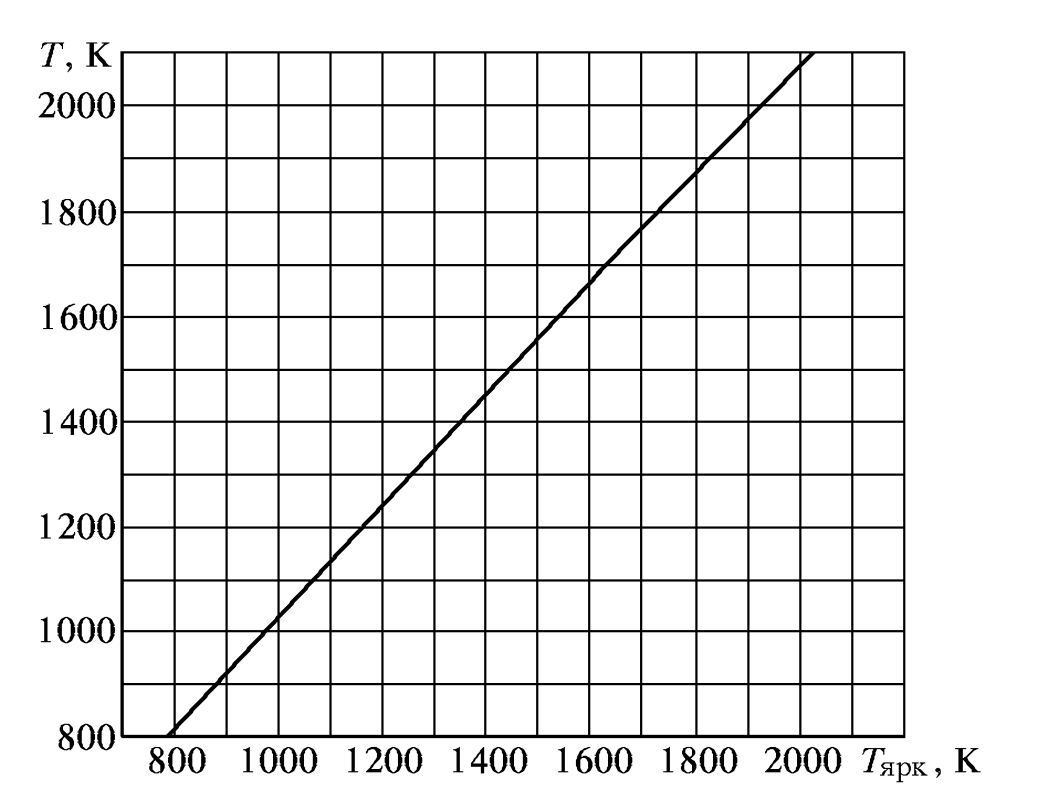
\includegraphics[width = 14 cm]{images/wolfram_real_temp_brigh_temp.png}
        \caption{График зависимости реальной температуры вольфрама от яркостной}
        \label{img:wolfram_real_temp_brigh_temp}
    \end{figure}
	
    Реальные тела не излучают как абсолютно чёрные. Если предположить, что спектральная излучательная способность исследуемого тела в $\varepsilon_T$ раз меньше спектральной излучательной способности АЧТ (\ref{eq:stefan_boltzman_law}), то излучаемая телом интегральная мощность будет вычисляться по формуле:
    \begin{equation}
        W = \varepsilon_T S \sigma T^4
        \label{eq:grey_stefan_boltzmann}
    \end{equation}
    где $S$ -- площадь излучающей поверхности тела, $\sigma$ -- постоянная Стефана-Больцмана. В данном соотношении учтено, что температура окружающей нить среды много меньше температуры нити. Тела, которые описываются такой моделью называются \textit{серыми}. Вольфрам лучше всего описывается моделью серого тела при высоких температурах $T > 1500 \cels$. 
	
    Для проверки закона Стефана-Больцмана предполагается степенная зависимость мощности излучения от температуры $W \propto T^n$ в законе (\ref{eq:grey_stefan_boltzmann}). По экспериментальным данным строится график зависимости мощности излучения от температуры в двойном логарифмическом масштабе, и находится коэффициент наклона прямой, равный показателю степени $n$:
    
    \begin{equation}
        \ln W = \ln (\varepsilon_T S \sigma) + n \ln T
        \label{eq:lin_grey_stefan_boltzmann}
    \end{equation}
    
    При определении показателя степени $n$ зависимостью $\varepsilon_T$ от температуры пренебрегаем. При определении постоянной Стефана-Больцмана зависимостью $\varepsilon_T(T)$ пренебречь нельзя, поэтому для каждого значения температуры вычисляется своя $\sigma$:
    
    \begin{equation}
        \sigma = \frac{W}{\varepsilon_T(T) \cdot S \cdot T^4}
        \label{eq:calc_const_stefan_boltzman}
    \end{equation}
    
    Преобразовав выражение (\ref{eq:const_stefan_boltzmann}), можно получить формулу для определения постоянной Планка:
    \begin{equation}
        h = \sqrt[3]{\frac{2 \pi^5 k_Б^4}{15 c^2 \sigma}}
        \label{eq:calc_const_planck}
    \end{equation}

    \newpage
	
    \section{Результаты измерений и обработка данных}

    \subsection{Изучение работы оптического пирометра}

    С помощью пирометра измерим температуры модели АЧТ и проведём сравнение её значения со значением температуры, измеренной при помощи термопары. Изменяя ток через нить пирометра, добьёмся исчезновения нити на фоне изображения раскалённой поверхности дна АЧТ. Проверим корректность измерений: температура на пирометре не должна сильно отличаться от температуры АЧТ, измеренной термопарой. Проведя несколько измерений убедились, что значения отличаются не более, чем на $5\%$.
	
    \subsection{Измерение яркостной температуры накаленных тел}

    В опыте наблюдалось, что разные тела, накалённые до одинаковой термодинамической температуры, имеют различную яркостную температуру вследствие того, что разные материалы имеют разный спектральный коэффициент поглощения.
 
    \subsection{Проверка закона Стефана-Больцмана}

    Результаты измерения яркостной температуры вольфрамовой нити $T$ при различной подаваемой на неё мощности $W$ приведены в таблице \ref{table:stefan_boltzmann}.
    
    \begin{table}[H]
        \centering
        \addtolength{\tabcolsep}{-4pt}
        \footnotesize
        \begin{tabular}{ccccc}
            \toprule
            $T_\text{ярк}, $ & $T$, K & $I$, А & $V$, В & $W$, Вт \\
            \midrule
            963  & 1236 & 0.56 & 2.12 & 1.19 \\
            1020 & 1293 & 0.58 & 2.27 & 1.32 \\
            1057 & 1330 & 0.57 & 2.19 & 1.25 \\
            1102 & 1375 & 0.59 & 2.39 & 1.41 \\
            1198 & 1471 & 0.64 & 2.88 & 1.84 \\
            1288 & 1561 & 0.69 & 3.40 & 2.33 \\
            1359 & 1632 & 0.71 & 3.98 & 2.83 \\
            1424 & 1697 & 0.75 & 4.17 & 3.13 \\
            1491 & 1764 & 0.79 & 4.80 & 3.81 \\
            1556 & 1829 & 0.84 & 5.22 & 4.37 \\
            1613 & 1886 & 0.85 & 6.31 & 5.38 \\
            1690 & 1963 & 0.89 & 6.77 & 6.02 \\
            1750 & 2023 & 0.99 & 7.36 & 7.30 \\
            1812 & 2085 & 1.01 & 8.07 & 8.17 \\
            1897 & 2170 & 1.10 & 8.95 & 9.83 \\
            \bottomrule
        \end{tabular}
        \caption{Результаты измерения яркостной температуры вольфрамовой нити $T$ при различной подаваемой на неё мощности $W$}
	\label{table:stefan_boltzmann}
    \end{table}

    Измеренная яркостная температура преобразуется в термодинамическую температуру с помощью графика зависимости, изображённого на рисунке \ref{img:wolfram_real_temp_brigh_temp}. По результатам измерений построим график зависимости потока излучения от температуры в обычном (рис. \ref{fig:wt}) и двойном логарифмическом масштабах (рис. \ref{fig:lnw_lnt}).
	
    \begin{figure}[H]
        \centering
        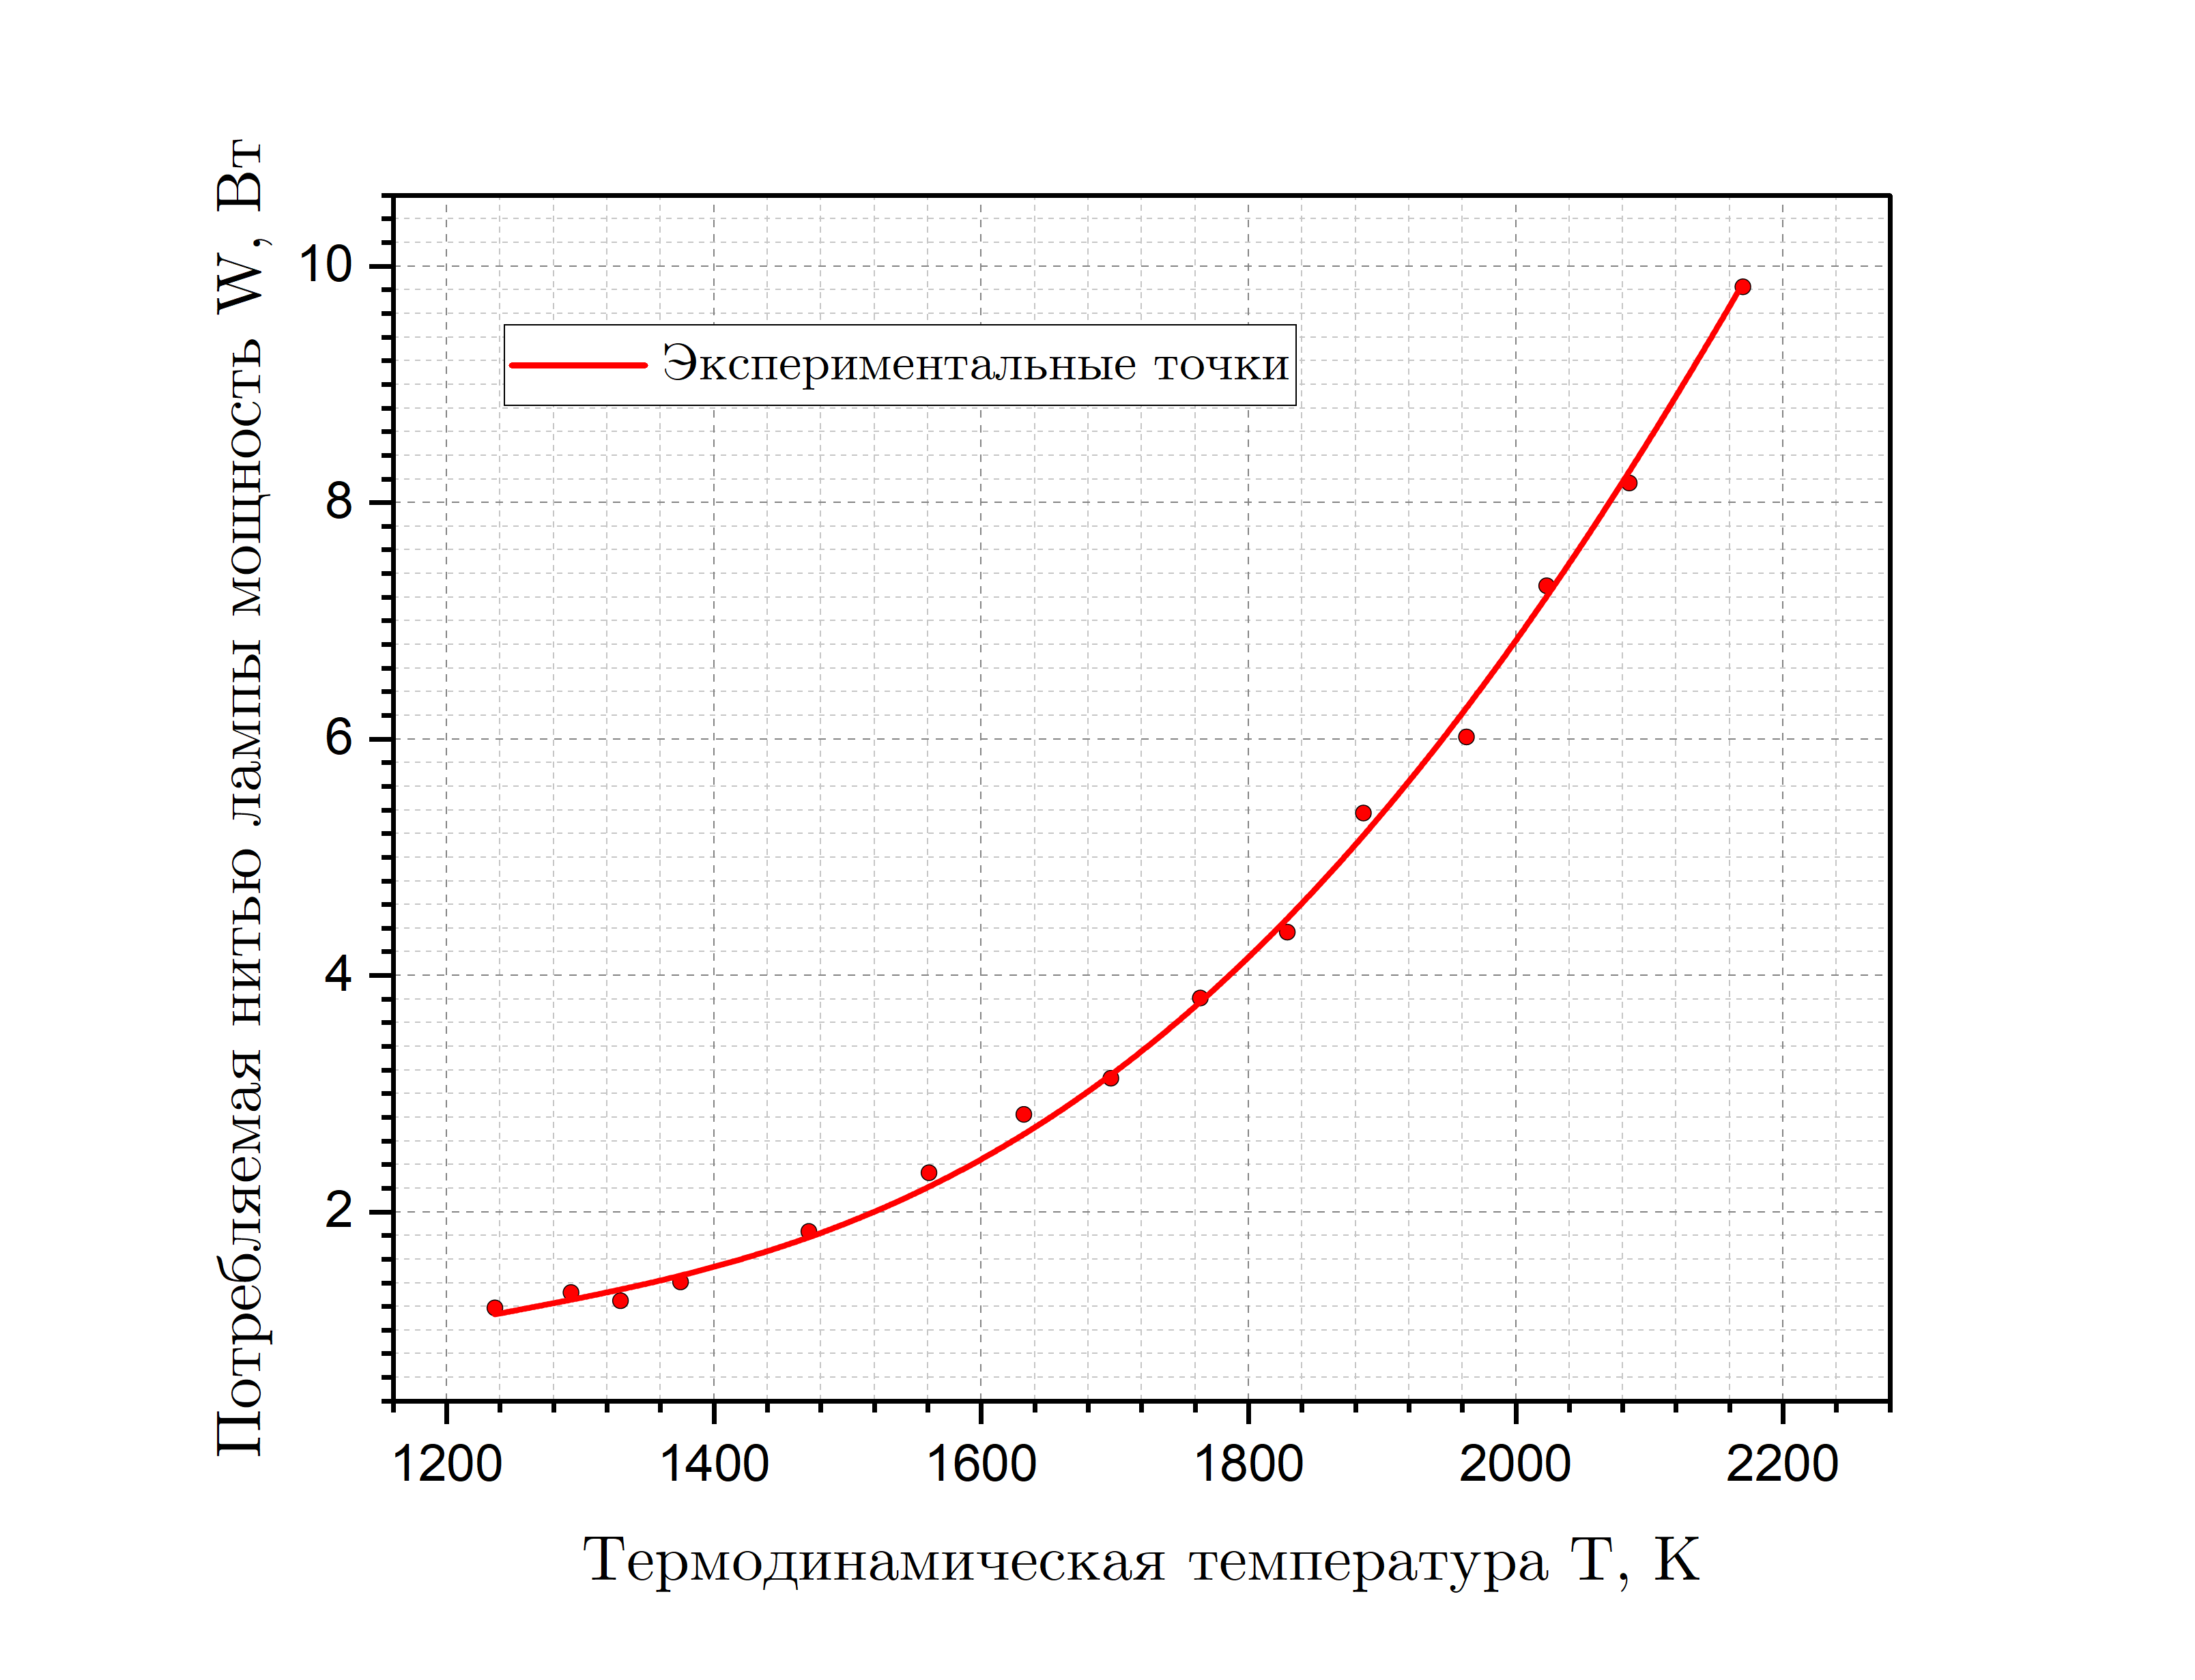
\includegraphics[width = 14 cm]{images/graph_W_T.png}
        \caption{Зависимость потока излучения от температуры $W(T)$}
        \label{fig:wt}
    \end{figure}

    \begin{figure}[H]
        \centering
        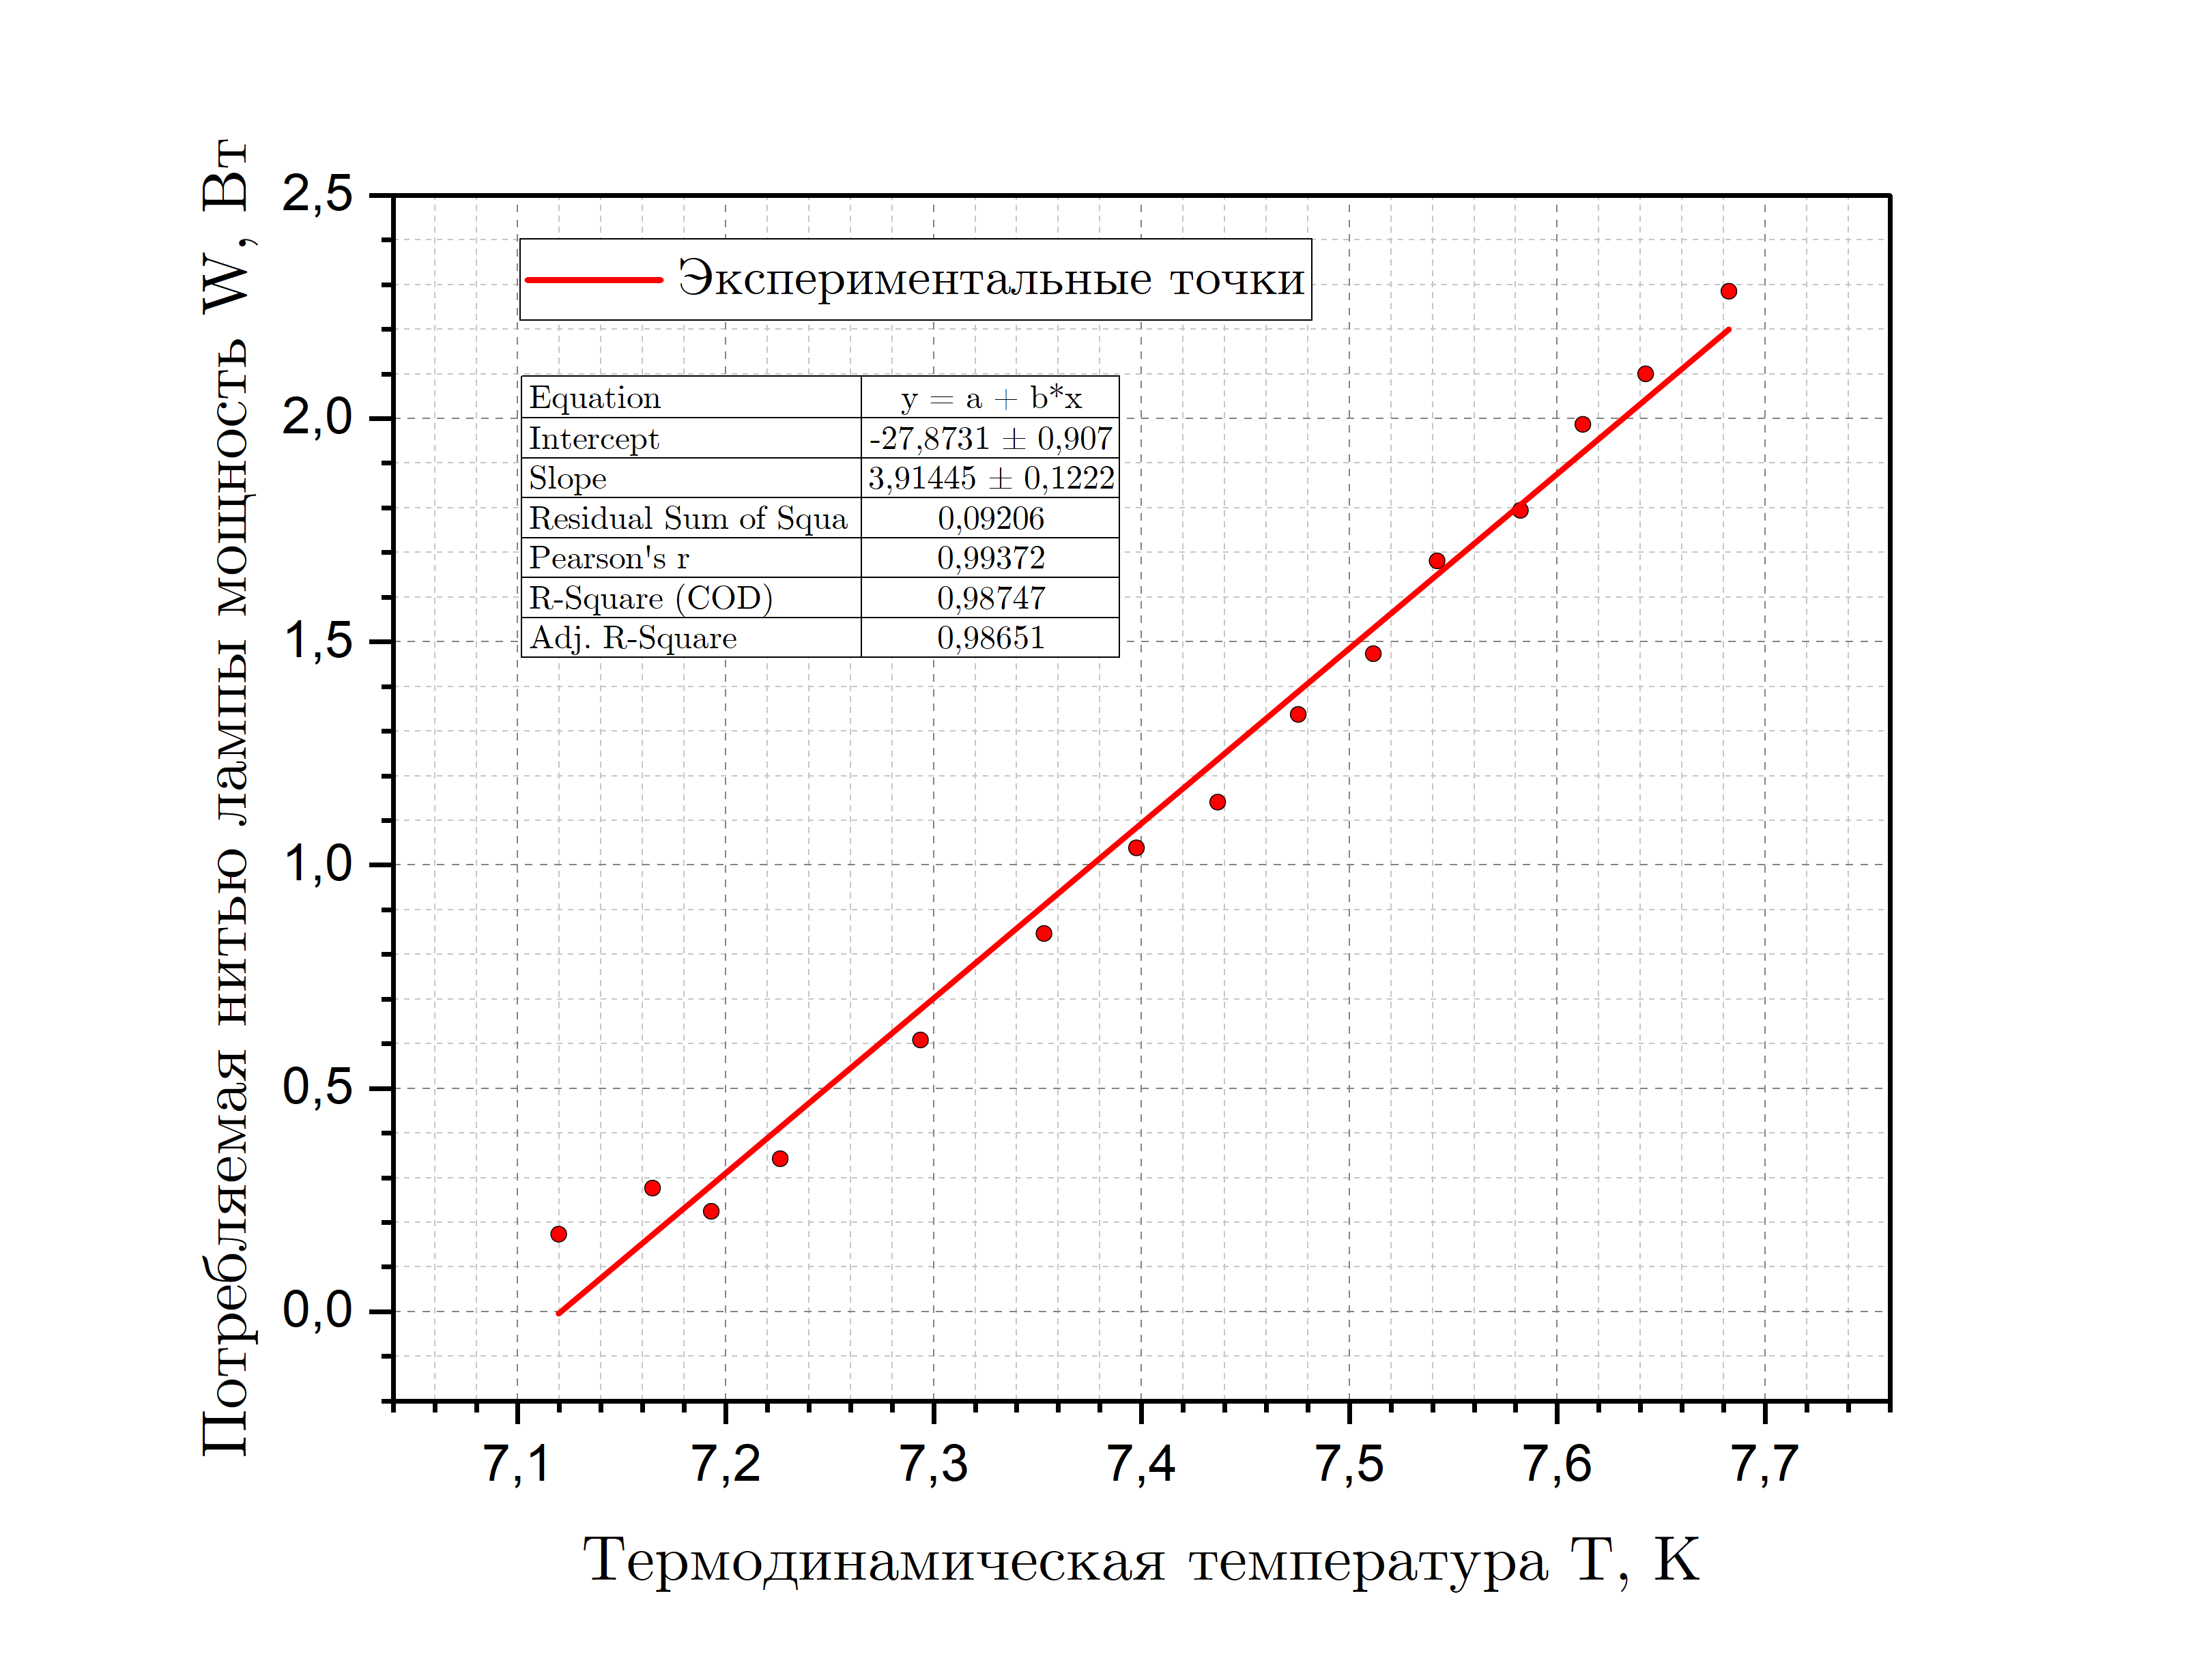
\includegraphics[width = 14 cm]{images/graph_ln_W_T.png}
        \caption{Зависимость потока излучения от температуры $W(T)$ в двойном логарифмическом масштабе}
        \label{fig:lnw_lnt}
    \end{figure}
	
    На графике в двойном логарифмическом масштабе аппроксимируем результаты измерений прямой $\ln W = b + n \ln T$ с помощью метода наименьших квадратов и определим показатель степени температуры $n$ в законе Стефана-Больцмана согласно формулы \ref{eq:lin_grey_stefan_boltzmann}. Коэффициенты МНК: \\
    $$n = 3.9 \pm 0.1,\;\; b = -28 \pm 1.$$

    Найдём величину постоянной Стефана-Больцмана по формуле (\ref{eq:calc_const_stefan_boltzman}) для каждого измеренного значения $T$, превышающего $1700$ K, где $S = 0,36 \text{ см}^2$ -- эффективная площадь излучающей поверхности нити лампы при температуре более $1500 \cels$. Результаты приведены в таблице \ref{table:calc_const_stefan_boltzman}.

     \begin{table}[H]
        \centering
        \footnotesize
        \begin{tabular}{ccccc}
            \toprule
            $T$, K & $W$, Вт & $\varepsilon_T$ & $\sigma \cdot 10^{-12}$, $\frac{\text{Вт}}{\text{см}^2 \cdot \text{К}^4}$ & $\Delta_\sigma \cdot 10^{-12}$,$ \frac{\text{Вт}}{\text{см}^2 \cdot \text{К}^4}$ \\
            \midrule
            1764 & 3.81 & 0.209 & 5.2 & 0.5 \\
            1829 & 4.37 & 0.223 & 4.8 & 0.5 \\
            1886 & 5.38 & 0.236 & 5.0 & 0.5 \\
            1963 & 6.02 & 0.236 & 4.7 & 0.5 \\
            2023 & 7.30 & 0.249 & 4.9 & 0.5 \\
            2085 & 8.17 & 0.249 & 4.8 & 0.5 \\
            2170 & 9.83 & 0.249 & 4.9 & 0.5 \\
            \bottomrule
        \end{tabular}
        \caption{Результаты измерений постоянной Стефана-Больцмана}
	\label{table:calc_const_stefan_boltzman}
    \end{table}

    Погрешность же, по правилам оценки погрешностей косвенных вычислений, можно оценить суммой относительных ошибок каждой величины:
    $$\varepsilon_\sigma \approx \sqrt{\varepsilon_S^2 + (4\varepsilon_T)^2} \sim 10 \%. $$\\

    Для вычисления постоянной Планка по формуле (\ref{eq:calc_const_planck}), определим постоянную Стефана-Больцмана, усреднив $\sigma_i$ для температур $T > 1700\; K$
    
    $$ \sigma = (4.9 \pm 0.5) \cdot 10^{-12} \: \frac{\text{Вт}}{\text{cм}^2 \cdot K}.$$
	
    Погрешность постоянной Планка можно оценить по правилам нахождения погрешностей косвенных измерений:
	
    $$\varepsilon_h \approx \frac{1}{3} \varepsilon_\sigma.$$

    $$ h = (6.9 \pm 0.2) \cdot 10^{-34} \: \text{Дж} \cdot \text{с}.$$

    \subsection{Измерение "яркостной температуры" неоновой лампочки}

    Термодинамическая температура неоновой лампочки равна комнатной, и не соответствует её яркостной температуре ($\sim 850 \cels$) вследствие того, что неоновая лампочка не является моделью абсолютно чёрного или серого тела, и её излучение носит совершенно другую природу.

    \section{Заключение}
    
    В работе был экспериментально проверен закон Стефана-Больцмана. В пределах погрешности показатель степени температуры $n$ сходится с теоретическим значением:
    $$
    n = (3.9 \pm 0.1).
    $$

    Были определены постоянные Стефана-Больцмана $\sigma$ и Планка $h$. 
    $$
    \sigma = (4.9 \pm 0.5) \cdot 10^{-12} \frac{\text{Вт}}{\text{см}^2 \cdot K},$$ 
    $$h = (6.9 \pm 0.2) \cdot 10^{-34}\; \text{Дж} \cdot \text{с}.$$

    Измеренные постоянные по порядку сходятся с теоретическими значениями.
    
\end{document}